\documentclass{article}
\usepackage[margin=1in]{geometry}

\usepackage{listings}
\usepackage{upquote}
\usepackage{xcolor}
\usepackage{ulem}

\usepackage{zi4}

\usepackage{tikz}
\usetikzlibrary{arrows}
\usetikzlibrary{tikzmark}
\usetikzlibrary{calc}%
\usetikzlibrary{positioning,fit,backgrounds,decorations.pathmorphing}
\usetikzlibrary{intersections}
\usetikzlibrary{shapes}

\pagestyle{empty}
\begin{document}

\lstdefinestyle{JavaSource}{
  basicstyle=\ttfamily,
  language=Java,
  showstringspaces=false,  
  % framexleftmargin=20pt,  
  keepspaces=true,
  % frame=single,
}

\lstdefinestyle{JavaError}{
  basicstyle=\small\ttfamily,
}

\begin{lstlisting}[style=JavaSource,escapeinside={(*}{*)}]
1 class Melon {
2     (*\tikzmark{a}*)final int i(*\tikzmark{b}*);
3 
4     (*\tikzmark{e}*)Melon(boolean b) {(*\tikzmark{f}*)
5         if (b)(*\tikzmark{k1}*)
6             (*\tikzmark{c}*)i = 3(*\tikzmark{d}*);(*\tikzmark{k2}*)
7     }(*\tikzmark{k3}*)
8 }
\end{lstlisting}

\begin{tikzpicture}
[remember picture,enum/.style={circle,draw=gray,very
    thin,fill=black,text=white,inner sep=1pt}]

  % Box for final i
  \coordinate[overlay] (final i top left) at
    ($(pic cs:a) + (-0.1em, 0.9em)$);

  \coordinate[overlay] (final i bottom right) at
    ($(pic cs:b) + (0.1em,-0.3em)$);

  \path[overlay] let \p1=(final i top left), 
    \p2=(final i bottom right) in
      coordinate (final i left mid) 
        at ($(\x1, \y1)!0.5!(\x1, \y2)$);

  \draw[fill opacity=0.3,fill=green!50,overlay,rounded corners]   
    (final i top left) rectangle 
    (final i bottom right);

  % Box for i = 3
  \coordinate[overlay] (i 3 top left) at
    ($(pic cs:c) + (-0.1em, 0.9em)$);

  \coordinate[overlay] (i 3 bottom right) at
    ($(pic cs:d) + (0.1em,-0.3em)$);

  \path[overlay] let \p1=(i 3 top left), 
    \p2=(i 3 bottom right) in
      coordinate (i 3 left mid) 
        at ($(\x1, \y1)!0.5!(\x1, \y2)$);

  \path[overlay] let \p1=(i 3 top left), 
    \p2=(i 3 bottom right) in
      coordinate (i 3 bottom mid) 
        at ($(\x1, \y2)!0.5!(\x2, \y2)$);

  \draw[fill opacity=0.3,fill=red!50,overlay,rounded corners]   
    (i 3 top left) rectangle 
    (i 3 bottom right);

  \draw[overlay,>=latex,->] (final i left mid) -- +(-2em, 0) |- (i 3 left mid);

  % Melon(boolean b) coordinates
  \coordinate[overlay] (melon top left) at
    ($(pic cs:e) + (-0.1em, 0.9em)$);

  \coordinate[overlay] (melon bottom right) at
    ($(pic cs:f) + (0.1em,-0.3em)$);

  \path[overlay] let \p1=(melon top left), 
    \p2=(melon bottom right) in
      coordinate (melon right mid) 
        at ($(\x2, \y1)!0.5!(\x2, \y2)$);

  % Enumerate
  \node[overlay,enum] (node 1) at ($(melon right mid) + (1em,0em)$) {\tiny 1};
  \node[overlay,enum] (node 2) at ($(melon right mid) + (7em,0em)$) {\tiny 2};
  % \node[overlay,enum] at ($(c mid) + (7em,-2em)$) {\tiny 2};

  % Line
  \draw[overlay,>=square,->,draw=green!50,fill=green!50]    
      ($(node 1.south) + (0,-1em)$) -- +(-3em, 0em);
  \draw[overlay,>=square,->,draw=green!50,fill=green!50]
    ($(node 1.south) + (0,-2em)$) -- +(-3em, 0em);
  \draw[overlay,>=square,->,draw=green!50,fill=green!50] 
    ($(node 1.south) + (0,-3em)$) -- +(-3em, 0em);
  \draw[overlay] (node 1.south) -- +(0,-4em);

  \draw[overlay,>=square,->,draw=green!50,fill=green!50] 
    ($(node 2.south) + (0,-1em)$) -- +(-3em, 0em);
  \draw[overlay,>=square,->,draw=red!50,fill=red!50] 
    ($(node 2.south) + (0,-2em)$) -- +(-3em, 0em);
  \draw[overlay,>=square,->,draw=green!50,fill=green!50] 
    ($(node 2.south) + (0,-3em)$) -- +(-3em, 0em);
  \draw[overlay] (node 2.south) -- +(0,-4em);

  \node[overlay,rectangle,draw=black,fill=gray!10,dashed] (exp) at 
    ($(node 1.south) + (0,-4.5em)$) {\small\texttt{i = 3}};

  \node[overlay,rectangle,draw=black,fill=gray!10,dashed] at 
    ($(node 2.south) + (0,-4.5em)$) {\small\texttt{i = ?}};

  \node[overlay,rectangle,draw=black,fill=gray!10,dashed] at 
    ($(node 1.north) + (0,1em)$) {\small\texttt{b =  true}};

  \node[overlay,rectangle,draw=black,fill=gray!10,dashed] at 
    ($(node 2.north) + (0,1em)$) {\small\texttt{b =  false}};

  \draw[overlay,>=latex,->] (i 3 bottom mid) |- (exp.west);


  % \node[overlay,rectangle,draw=black,fill=gray!10,dashed,right] at ($(c mid)
  % + (8em,-2em)$) {\small\texttt{m((double) 1, (int) 2);}};
 
\end{tikzpicture}

\end{document}
